\documentclass[border=10pt]{standalone}
\usepackage{tikz}
\usetikzlibrary{arrows.meta}
\begin{document}
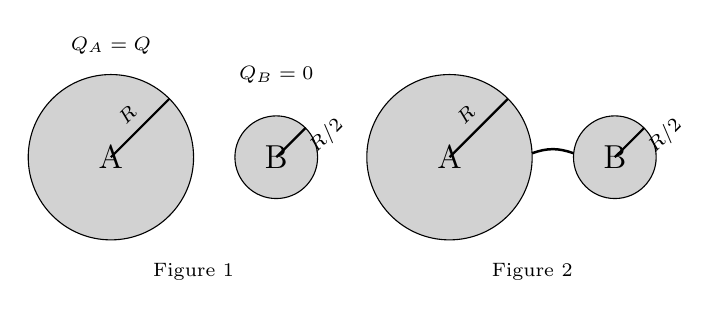
\begin{tikzpicture}[>=Stealth, scale=1.0, every node/.style={font=\scriptsize}]
  % ================= Figure 1: isolated spheres =================
  \fill[gray!35] (-3.4,0) circle (1.05);
  \draw (-3.4,0) circle (1.05);
  \node at (-3.4,0) {\large A};
  \draw[line width=0.8pt] (-3.4,0) -- (-2.657,0.743) node[midway, above, sloped, yshift=0.02cm] {$R$};
  \node at (-3.4,1.42) {$Q_A = Q$};

  \fill[gray!35] (-1.3,0) circle (0.525);
  \draw (-1.3,0) circle (0.525);
  \node at (-1.3,0) {\large B};
  \draw[line width=0.8pt] (-1.3,0) -- (-0.928,0.371) node[pos=1.22, below, sloped, yshift=-0.01cm] {$R/2$};
  \node at (-1.3,1.05) {$Q_B = 0$};

  \node at (-2.35,-1.45) {Figure 1};

  % ================= Figure 2: connected by wire =================
  \fill[gray!35] (0.9,0) circle (1.05);
  \draw (0.9,0) circle (1.05);
  \node at (0.9,0) {\large A};
  \draw[line width=0.8pt] (0.9,0) -- (1.643,0.743) node[midway, above, sloped, yshift=0.02cm] {$R$};

  \fill[gray!35] (3.0,0) circle (0.525);
  \draw (3.0,0) circle (0.525);
  \node at (3.0,0) {\large B};
  \draw[line width=0.8pt] (3.0,0) -- (3.372,0.371) node[pos=1.22, below, sloped, yshift=-0.01cm] {$R/2$};

  % wire between the spheres
  \draw[line width=0.9pt] (1.95,0.05) to[bend left=20] (2.475,0.05);

  \node at (1.95,-1.45) {Figure 2};
\end{tikzpicture}
\end{document}
